
\documentclass[journal,UTF8]{IEEEtran}
\usepackage{ctex}
\usepackage{color}

%
\usepackage{cite}

\ifCLASSINFOpdf
 \usepackage[pdftex]{graphicx}
  % declare the path(s) where your graphic files are
 \graphicspath{{../pdf/}{../jpeg/}}
  % and their extensions so you won't have to specify these with
  % every instance of \includegraphics
\DeclareGraphicsExtensions{.pdf,.jpeg,.png}
\else
  % or other class option (dvipsone, dvipdf, if not using dvips). graphicx
  % will default to the driver specified in the system graphics.cfg if no
  % driver is specified.
\usepackage[dvips]{graphicx}
  % declare the path(s) where your graphic files are
\graphicspath{{../eps/}}
  % and their extensions so you won't have to specify these with
  % every instance of \includegraphics
\DeclareGraphicsExtensions{.eps}
\fi

\usepackage[cmex10]{amsmath}

%\usepackage{algorithmic}
\usepackage[ruled]{algorithm2e}
\usepackage{array}

\ifCLASSOPTIONcompsoc
  \usepackage[caption=false,font=normalsize,labelfont=sf,textfont=sf]{subfig}
\else
  \usepackage[caption=false,font=footnotesize]{subfig}
\fi

\hyphenation{op-tical net-works semi-conduc-tor}



\begin{document}
%
% paper title
% can use linebreaks \\ within to get better formatting as desired
% Do not put math or special symbols in the title.
\title{A VCA Protocol Based Multi-level Flexible Architecture on Embedded PLCs for Visual Servo Control }

\maketitle


\begin{abstract}

% ^.
\end{abstract}

% Note that keywords are not normally used for peerreview papers.
\begin{IEEEkeywords}
motion control, visual servo control, embedded PLC, multi-level architecture
\end{IEEEkeywords}

% For peer review papers, you can put extra information on the cover
% page as needed:
% \ifCLASSOPTIONpeerreview
% \begin{center} \bfseries EDICS Category: 3-BBND \end{center}
% \fi
%
% For peerreview papers, this IEEEtran command inserts a page break and
% creates the second title. It will be ignored for other modes.
\IEEEpeerreviewmaketitle



\section{Introduction}
Integration technologies 驱动着工业自动化的发展\cite{Kazmierkowski2007Integration}。对传感器,控制器,机器人,生产线以及软件工具的不断整合,催生了自省设备,智能工厂,CPS,等概念\cite{Wan2018An,Chekired2018Industrial}。最近的一些研究,\cite{Colombo2006An,Vaccaro2010An,Dean2017Integration}介绍了融合技术的发展。在工业自动化中,逻辑控制系统,运动控制系统和视觉系统具有重要作用,且密不可分\cite{Feng2002Integrating,Chang2006Motion,Feng2005Practical}。另一方面,边缘计算,雾计算,边缘人工智能等新技术的发展\cite{Hu2017Fog,Hou2018Green,PaceAn},也对逻辑逻辑控制系统,运动控制系统和视觉系统等相关边缘设备提出了新的要求。

\subsection{Motivations}
%Nowdays, visual system has been applied in various fields.
%
%On the other hand, according to the reliablity and \cite{Hossain2014Advanced}, Lots of papers are focusing on it, \cite{Jiang2013System,Jiang2013Bayesian} guarantee the reliability by verifying the program of PLCs, \cite{Gerk2006Advanced,Chang2007Adaptive,Dominic2016PLC} improve the performance of PLCs using advanced algorithms, \cite{wu2018customized} alleviates the development complexity of PLCs with a special software structure, \cite{Sch2013Development,Morenas2017Shop} pose methods to update PLC programs dynamically.
%
%Motion control is a key technology\cite{Ohnishi2002Motion} of automation. It drives various types of equipments to replace tremendous labors. Since advanced in algorithms, in
Nowdays, visual system has been applied in various fields. The logic control on PLC has wide applications. Motion control 
\cite{Chen2014A} is a typical case that describes how the three parts collaborate. The visual system analyzes the context and get error put into the motion system. Simultaneously the logic program are judging the information, such as the position limitation of the every axis. Hence, how to pose a flexible structure to the integration of logic control system, servo system and visual system, guides us.





\subsection{Related Works}

视觉控制系统均是由专用控制系统和视觉系统组成。例如搬运\cite{Xing2014Intersection},,电路检测\cite{Nian2005An},分拣系统,welding\cite{Chen2014A},装配\cite{Wang2008Visual,Xiao2014Visual},教育,robot\cite{Wu2013Cloud,Tsai2017A},unmanned aerial vehicles\cite{Guenard2010A,Serra2016Landing}。这些研究都很好的解决了各自领域的问题,但是这些方案都是基于视觉系统和专用控制系统完成。

例如\cite{Wu2013Cloud,Tsai2017A}中均使用机器人专用控制系统和视觉系统完成,在\cite{Guenard2010A,Serra2016Landing}中,使用无人机专用控制系统和视觉系统完成。\cite{Nian2005An}中,通过专用运动控制卡和视觉系统实现电路检测。

On the other hand. The integration of logic control and motion control has variously deep researches \cite{Ioannides2004Design,Shi2016The,Fang2017Design, syaichu2011model}. \cite{Ioannides2004Design,syaichu2011model} realize the motion control directly in PLC. \cite{Peng2011Linear, Qian2014A, OMRON2006CS1W} use motion control module collaborated with PLC to implement their applications. However, the development method in these papers is disordered. Therefore, in 2005, PLCopen organization has released a related standard \cite{PLCopen2005Function} which standardizes the motion control in PLC. Based on this standardization, \cite{S2006Advanced} provides an advanced implementation in distributed automation system and companies, such as 3S \cite{3S2017Logic}, provide some tools. \cite{wu2018customized} poses a customized real-time compilation method to reduce the development complexity.

Above works provide impressive integrations on visual servo control system and PLC with motion control functions, however there are few papers discussing the integration of visual system, motion control and PLC. Most of applications are focusing on its application with three individual system, such as \cite{Chen2014A}. Hence, an integration structure of logic control system, servo system and visual system should be provided to reduce the complexity and expand the application fields.

\subsection{Our Contributions}
我们提出了一种基于VCA协议的ePLC和视觉系统的柔性架构整合方案,来实现视觉私服控制。VCA协议描述了从视觉系统中获取数据后的组帧和在ePLC中数据帧在各层中的解析,从而实现视觉系统和ePLC的整合。ePLC硬件上的一种定制化设计,软件架构上的三层设计以及融合其中的VCA协议使得整个视觉私服系统变成一种柔性结构。

在接下来的部分中,\ref{SystemStructure}会介绍系统组成,包括硬件结构,软件结构,线程结构和内存设计。\ref{Integration}会介绍ePLC如何与视觉系统融合,包括VCA协议,PLC接口和视觉接口介绍。\ref{Execution}介绍系统执行过程,包括视觉层执行过程,逻辑层执行过程,算法层执行过程和多线程执行。\ref{Case}中介绍了两个例子,带视觉检测的绕线机和双目接球机器人。

\section{系统结构}
\label{SystemStructure}
\subsection{硬件结构}
硬件架构由嵌入式PLC系统和视觉系统组成。嵌入式PLC采用定制化结构,处理器以及外部资源例如数字量输入输出,模拟量输入输出和私服系统控制数量可根据需要定制等。图\ref{fig:Hardware}显示了一种典型的ePLC系统,采用双处理器架构,主从处理器之间通过共享内存通信。ePLC系统和视觉系统之间可以采用合适的已有通信方式,例如TCP/IP,Modbus,CAN等。图示采用了CAN通信。

\begin{figure}
	\centering
	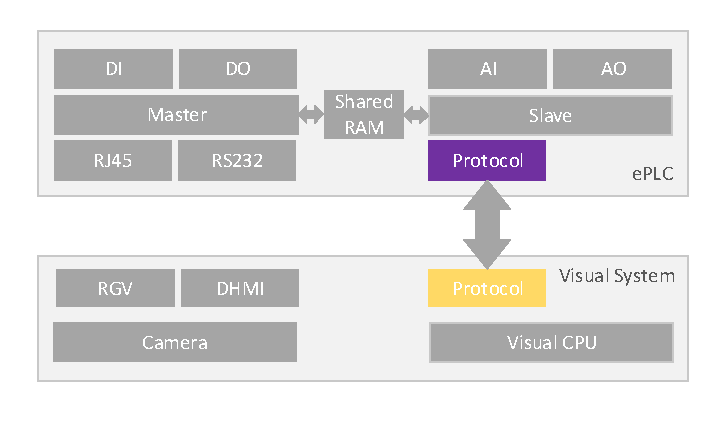
\includegraphics[width=3.5in]{fig/Hardware.pdf}
	\caption{ePLC 和视觉系统融合的硬件架构,ePLC采用双处理器的主从结构并和视觉系统通过CAN总线通信。}
	\label{fig:Hardware}
\end{figure}
\subsection{软件结构}
通常我们要实现视觉控制系统的典型软件架构如图\ref{fig:Software}左侧所示,通过逻辑程序连接各控制算法组成模块,在通过逻辑关系根据视觉系统的获取信息来连接各模块执行。这种设计通常会将视觉处理,逻辑处理和控制算法混在一起编程,造成混乱。我们通过VCA协议实现算法层,逻辑层和视觉层的三层架构。软件结构设计成图\ref{fig:Software}右侧所示结构。算法程序完成相关算法。逻辑程序处理算法间逻辑关系并调用相关算法。视觉程序解析视觉数据,调用模块执行。


\begin{figure}
	\centering
	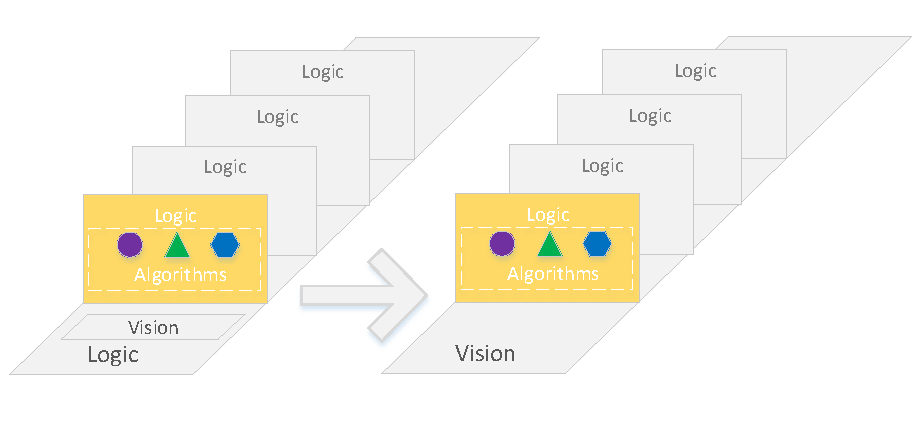
\includegraphics[width=3.5in]{fig/Software.pdf}
	\caption{The three-layer architecture of ePLC}
	\label{fig:Software}
\end{figure}
%%%Fig.4. The three-layer architecture of embed PLC.



\subsection{线程结构}
我们采用了\cite{wu2018customized}中类似的线程结构。我们特别强调以下三个线程:
\begin{enumerate}
	\item Visual Thread. 视觉线程,该线程主要完成视觉层协议解析,和逻辑层数据交互和模块调用。
	\item LC Thread. 逻辑线程,该线程主要完成逻辑程序处理,改成协议解析,和逻辑层和算法层之间数据交互和算法调用。
	\item Algorithm Thread. 算法线程,主要完成和逻辑层之间的数据交互和算法执行。
\end{enumerate}



\begin{figure}
	\centering
	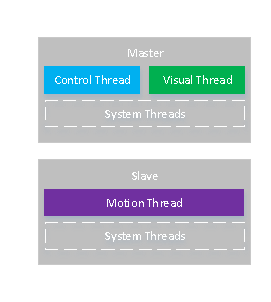
\includegraphics[width=3in]{fig/Threads.pdf}
	\caption{ The process of the three type threads}
	\label{fig:Threads}
\end{figure}
\subsection{内存设计}
在内存的PLC专用存储空间主要由位数据区(M区)和字节数据区(D区)组成。整个系统的PLC专用区分布在三个内存中:主控制器内存,主从共享内存和从控制器内存中。在我们的系统中规定了集合的两个属性如下:

\textbf{Definition 1} 集合 $S$ 具有 $\mathcal{B}$ 属性:$\exists (S=\{s_1,s_2,...,s_i,...s_n\}) \subset M$ and $(\forall s_{i} \in S) \in \{\mathcal{F}(s_i) = 0,\mathcal{O}(s_i) = 1\} $

\textbf{Definition 2} 集合 $S$ 具有 $\mathcal{D}$ 属性:$\exists (S=\{s_1,s_2,...,s_i,...s_n\}) \subset D$ and $\forall s_{i} \in S$ has 4 Byte。

其中$\mathcal{F}(s_i)$表示$s_i$中数据为0,$\mathcal{O}(s_i)$表示$s_i$中数据为1。

内存结构如图\ref{fig:RAM}所示。主要分三个部分,主处理器内存分配,共享内存分配,从处理器内存分配。各个分区作用介绍如下:
\begin{enumerate}
	\item LCF。该区域表示逻辑控制区。
	\item MPF。主到从数据传递标志区。
	\item LCD。逻辑数据存放区。
	\item VD。视觉数据存放区。存放从视觉系统传输过来的数据。
	\item MtoS。主到从数据存放区。
	\item StoM。从到主数据存放区。
	\item AF。算法标志区。
	\item AD。算法数据区。
	\item SPF。从到主传递标志区。
\end{enumerate}

 我们定义了主从处理器之间的数据交互方法为$\mathcal{P}$,如下:
\begin{equation}
\left\{
\begin{array}{l}
\mathcal{P}_{mts} =\mathcal{I} (ms_i,mc_i,mf_i,sa_i,sf_i,sd_i)\\
\mathcal{P}_{stm} =\mathcal{I} (ss_i,sd_i,sf_i,ma_i,mf_i,md_i)
\end{array}
\right.
\end{equation}
$\mathcal{P}_{mts}$和$\mathcal{P}_{mts}$具有相同执行函数$\mathcal{I}$,且执行过程如下:
$\mathcal{O}(ms_i)\to\mathcal{O}(mf_i)\to send(sd_i)\to\mathcal{O}(sf_i)\to check(sd_i)\to\mathcal{O}(sa_i)\to\mathcal{O}(mc_i)\to\mathcal{F}(ms_i)\to\mathcal{F}(mf_i)\to\mathcal{F}(mc_i)\to\mathcal{F}(sf_i)\to\mathcal{F}(sa_i)$
\begin{figure}
	\centering
	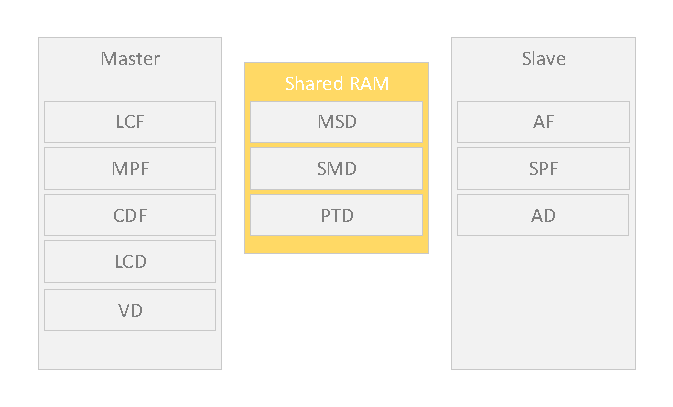
\includegraphics[width=3in]{fig/RAM.pdf}
	\caption{ The process of the three type threads}
	\label{fig:RAM}
\end{figure}

%%%Fig.6. Distribution of dedicated public data area.
\section{视觉控制系统融合}
\label{Integration}

\subsection{VCA Protocol Template}
In cater to most applications, we propose a VCA-based flexible architecture. As shown in Fig. , a protocol template ($PT$) is adopted to support various types of implementations and a $PT$ uniquely corresponds to a type of application. In the flexible architecture, users only need to redesign and reload the $PT$ and then they can reuse the visual servo system again. The $PT$ could be loaded into a stationary address of visual system and ePLC system. After restarting both systems, it will be put into a fixed area of RAM. The parsing modules form both systems will read it when parsing the protocol data.
 
 The $PT$ is defined below:
 \begin{equation}
 \left\{
 \begin{array}{l}
    PT = \{HPT, VLT, CLT, ALT\}\\
    HPT = \{CID, TDA\}\\
    VLT = \{MID, MAN, MSF, MDA, MAS, CDATA\}\\
    CLT = \{AID, APN, AF, ADA, APS, ADATA\}\\
    ALT = \{PID, PDATA\}
 \end{array}
 \right.
 \end{equation}
 
 The $PT$ contains four parts: head of protocol template ($HPT$), visual layer template ($VLT$), control layer template ($CLT$) and algorithm layer template ($ALT$). Every part explains as follows: 
 \begin{enumerate}
 	\item $HPT$: this part includes communication unique ID ($CID$), template data storage address ($TDA$). Every $PT$ only has one $HPT$.
 	\item $VLT$: it consists of module unique ID ($MID$), module contained algorithm number ($MAN$), module start flag ($MSF$), module data start address ($MDA$), module contained algorithm IDs ($MAS$) and control data ($CDATA$). $VLT$ is not $\emptyset$. Every $MAS$ include $MAN$ algorithm IDs. 
 	\item $CLT$: it is comprised of algorithm unique ID ($AID$), algorithm contained parameter number ($APN$), $AF$, algorithm data start address $ADA$, algorithm contained parameter IDs ($APS$) and algorithm data ($ADATA$). $CLT$ is not $\emptyset$.Every $APS$ include $APN$ parameter IDs.
 	\item $ALT$: it contains parameter unique ID ($PID$), parameter data ($PDATA$). $CLT$ is not $\emptyset$. 
 \end{enumerate}
 \subsection{VCA Protocol Frame}
 The VCA protocol frame $PF$ consists of visual frame, control frame and algorithm frame as shown in \ref{fig:Protocol}. We use the same name if the $PT$ and $PF$ both have the items.

 \begin{enumerate}
	\item Visual frame: it consists items of $MID$, $MSF$, $MDA$, visual frame length $VFL$, $CDATA$ and cyclic redundancy check $CRC$.The $CDATA$ contains several control frames.
	\item Control frame: it is comprised of $AID$, $AF$, $ADA$, control frame length ($CFL$) and $ADATA$.
	The $ADATA$ includes several algorithm frames. 
	\item Algorithm frame: it contains $PID$, $PDATA$. $PID$ is also the address of $PDATA$.
\end{enumerate}
\begin{figure}
	\centering
	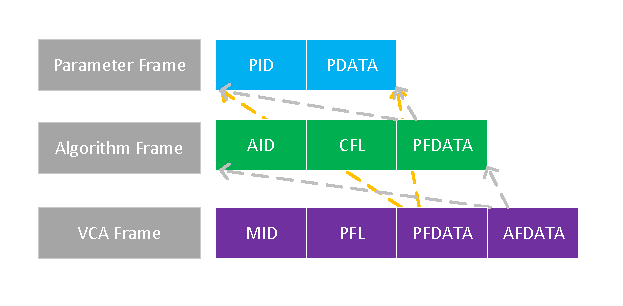
\includegraphics[width=3in]{fig/Protocol.pdf}
	\caption{ VCA Protocol.}
	\label{fig:Protocol}
\end{figure}
\subsection{PLC Interface}
The PLC interface is designed to transfer VCA protocol frame to PLC in $VS$. It has five steps: create data, $VL$ framing, $CL$ framing, $AL$ framing and transmission.

\textbf{Create date}: after image processing, the $VS$ extracts the useful data and storages into visual extracted data ($VED$) in which the parameters could be indexed by the $PID$.

\textbf{\emph{VL} Framing}: the process is realized as the Algorthm \ref{alg1}. It searches the $PT$ with $mid$ to find the relevant $vlt_x$. Through it, the $VS$ can obtain the $msf$ and $mda$. According to $man$, call the next step ($VL$ Framing) to gain the $cdata$. Then calculate the length ($vfl$) and $crc$ to finish the $VL$ framing.

\textbf{\emph{CL} Framing}: Algorthm \ref{alg2} illustrates the process. The $VS$ seeks the $FT$ to gain the $clt_y$ which contains the $af$ and $ada$. According to $apn$, call the next step ($AL$ Framing) to obtain the $cdata$ and then calculate the length ($cfl$) to finish the $CL$ framing.  

\textbf{\emph{AL} Framing}: Algorthm \ref{alg3} shows the process. The $VS$ obtains the $alt_z$ frome $FT$ and then combines the $pid$ and $pdata$.

\textbf{Transmission}: transfer the $VCA$ protocol frame to $ePLC$ with the relevant communication protocol in $CID$.

\begin{algorithm}
	\label{alg1}
	\caption{$VLFraming$}%算法名字
	%\LinesNumbered %要求显示行号
	\KwIn{$mid$, $VED$}%输入参数
	\KwOut{$vlf$}%输出
	Search the $PT$ with $mid$ and get $vlt_x$\;
	Create $vlf$ according to $vlt_x$\;
	\If{create successfully}{
		$vlf.mid$ = $vlt_x.mid$\;
		$vlf.msf$ = $vlt_x.msf$\;
		$vlf.mda$ = $vlt_x.mda$\;
	}
	\For{$i=0$;$i<vlt_x.man$;$i++$}{
		ALFraming($vlt_x$.$mas$[i], $VED$,$cdata$)\;
	}
    $vlf.cdata$ = $cdata$\; 
	$vlf.vfl$ = Length($vfl$)+4\;
	$vlf.crc$ = CRC16($vlf$)\;		 
\end{algorithm}

\begin{algorithm}
	\label{alg2}
	\caption{$CLFraming$}%算法名字
	%\LinesNumbered %要求显示行号
	\KwIn{$aid$, $VED$, $cdata$}%输入参数
	\KwOut{$cdata$}%输出
	Search the $PT$ with $aid$ and get $clt_y$\;
	Create $clf$ according to $clt_y$\;
	\If{create successfully}{
		$clf.aid$ = $clt_y.aid$\;
		$clf.af$ = $clt_y.af$\;
		$clf.ada$ = $clt_y.ada$\;
	}
	\For{$i=0$;$i<clt_y.apn$;$i++$}{
		ALFraming($clt_y$.$aps$[i], $visualData$, $pdata$)\;
	}
	$clf.cfl$ = Length($clf$)\;	
	$cdata$ += $clf$\;	 
\end{algorithm}
\begin{algorithm}
	\label{alg3}
	\caption{$ALFraming$}%算法名字
	%\LinesNumbered %要求显示行号
	\KwIn{$pid$, $VED$,$pdata$}%输入参数
	\KwOut{$pdata$}%输出
	Search the $PT$ with $pid$ and get $alt_z$\;
	Create $alf$ according to $alt_z$\;
	\If{create successfully}{
		$alf.pid$ = $alt_z.pid$\;
		$alf.pdata$ = $VED.pid$\;
	}
	$pdata$ += $alf$\;	 
\end{algorithm}

\subsection{Vision Interface}
Vision interface is in the ePLC designed to interact with the $VS$. It includes five parts: receiving $VCA$ protocol frame, saving it, $VL$ deframing, $CL$ deframing and $AL$ deframing.

\textbf{Receiving \emph{VCA} protocol frame}: according to the $CID$ in $PT$, the $ES$ chooses the communication protocol receives the frame form $VS$.

\textbf{Savint \emph{VCA} protocol frame}:  
ePLC中需要接收从视觉系统获得的数据。该接口主要包括两部分:数据接收和视觉层数据解析。

\textbf{数据接收}:包括双方系统规定,使用已有协议(TCP/IP,MODBUS,CAN等)传递数据。

\textbf{视觉层数据解析}:先对数据进行CRC校验,如果数据错误则丢弃数据并通知视觉系统。如果数据正确,根据VLA协议对接收到的数据进行视觉层协议解析,获取数据后通知。
\begin{figure}
	\centering
	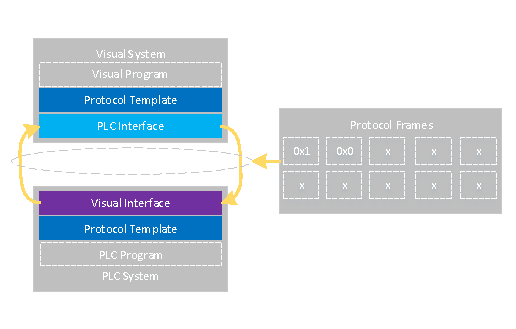
\includegraphics[width=3in]{fig/FlexibleLayer.pdf}
	\caption{ Data Interaction Based on VP Protocol.}
	\label{fig:FlexibleLayer}
\end{figure}
\begin{algorithm}
	\label{al4}
	\caption{$VLDeframing$}%算法名字
	%\LinesNumbered %要求显示行号
	\KwIn{$PDF$}%输入参数
    $mid \leftarrow$ four bytes start form $PDF$\;
    $msn \leftarrow$ four bytes start form $PDF+4$\; 
    $mda \leftarrow$ four bytes start form $PDF+8$\;
    $cdata \leftarrow$ $msn-12$ bytes start form $PDF+12$\;
	$CassMemM[mda]\leftarrow$ $cdata$\;
	$PDF\leftarrow$ $PDF+msn$\;
\end{algorithm}

\begin{algorithm}
	\label{al5}
	\caption{$CLDeframing$}%算法名字
	%\LinesNumbered %要求显示行号
	\KwIn{$mid$}%输入参数
	searchPT($mid$, $vlt_x$)\;
	$mda\leftarrow$ $vlt_x.mda$\;
	\For{$i=0$;$i<vlt_x.man$;$i++$}{
		searchPT($vlt_x.mas[i]$, $clt_y$)\;
		$CassMemS[clt_y.apa]\leftarrow$ $clt_y.apn \times 8$ bytes start form $mda$\; 
        $mda\leftarrow$ $mda+clt_y.apn \times 8$\;
	}
    clean\;
\end{algorithm}

\begin{algorithm}
	\label{al6}
	\caption{$ALDeframing$}%算法名字
	%\LinesNumbered %要求显示行号
	\KwIn{$aid$}%输入参数
	searchPT($aid$, $clt_y$)\;
	$ada\leftarrow$ $vlt_x.ada$\;
	\For{$i=0$;$i<clt_y.apn$;$i++$}{
		$CassMemA[CassMemA[ada]]\leftarrow$ $CassMemA[ada+4]$\;
		$ada\leftarrow ada+8$\;
	}
	clean\;
\end{algorithm}


\section{系统运行原理}
\label{Execution}
\subsection{视觉层的执行}
视觉层通过视觉接口和视觉执行模块两部分实现。通过视觉接口,从视觉系统中获取数据。视觉执行模块,通过执行顺序依次执行模块,并将视觉系统的数据不断反馈给逻辑层。



%\begin{figure}
%	\centering
%	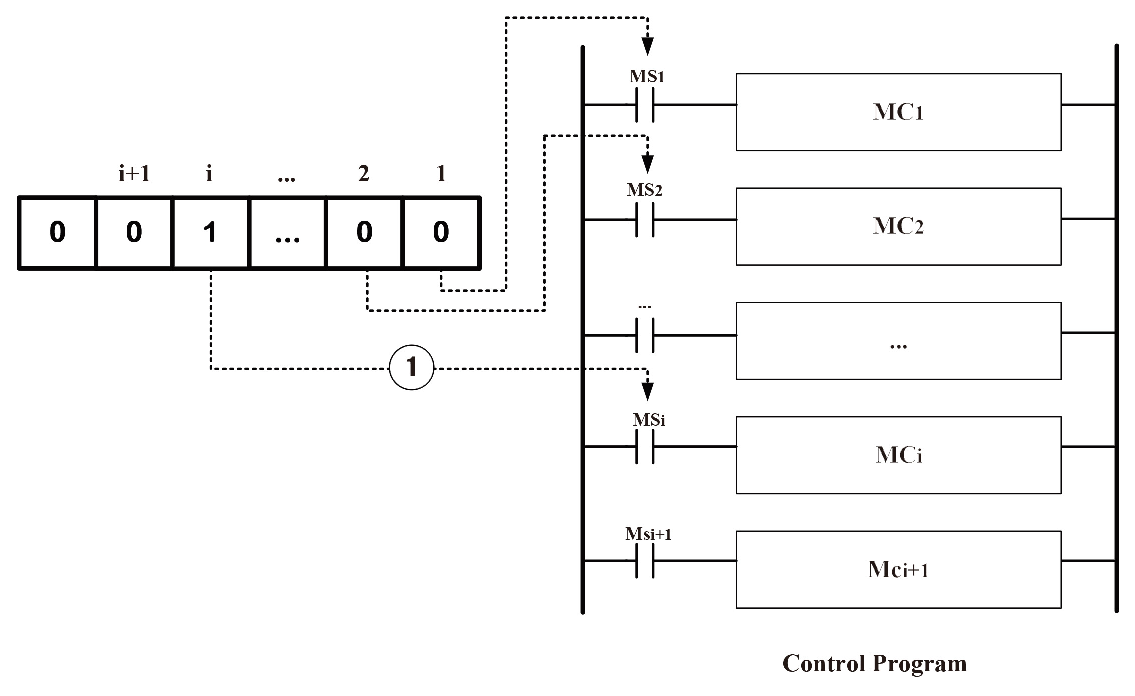
\includegraphics[width=3.5in]{fig/bitdatainM.eps}
%	\caption{Using bit data in the M area to control program module$\textquoteright$s execution}
%	\label{fig:bitdatainM}
%\end{figure}
%%%Fig.11. Using bit data in M area to control program module¡¯s execution.


\subsection{逻辑层执行}
逻辑层由模块数据初始化,逻辑程序,协议解析程序和数据交互程序组成。

当视觉层控制模块调用逻辑层模块执行时,先启动初始化程序初始化模块,运行逻辑程序,通过对视觉层给出的数据解析协议后,通过$\mathcal{P}_{mts}$方法将数据传递给引擎层,并一直获取从引擎层反馈的数据,如果算法执行完毕则清除所有标志位和状态。

%\begin{figure}
%\centering
%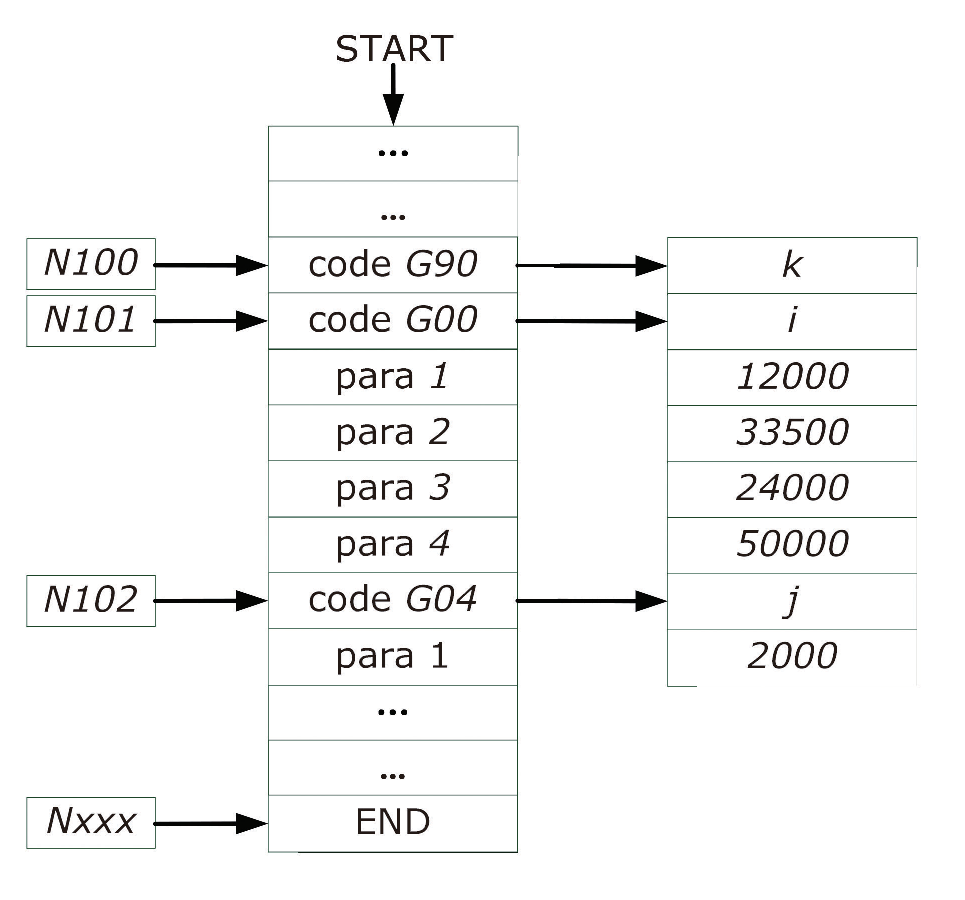
\includegraphics[width=3in]{fig/formatofCNCprogram.eps}
%\caption{The format of ACP program frame after compiling}
%\label{fig:formatofCNCprogram}
%\end{figure}
%%%Fig.8. The format of ACP program frame after compiling.




%%%Fig.9. The schematic of delivering ACP instruction parameters from ACPDD to ACPPSD

%\begin{figure}
%	\centering
%	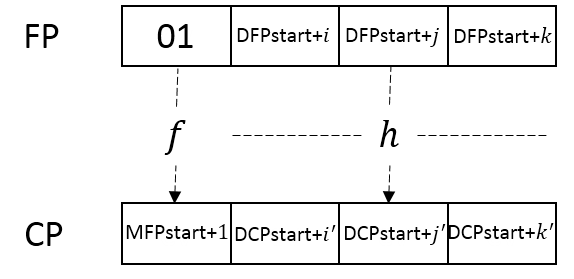
\includegraphics[width=2.5in]{fig/compilation.png}
%	\caption{ The compilation from flexible program to control program}
%	\label{fig:compilation}
%\end{figure}

%\begin{figure}
%	\centering
%	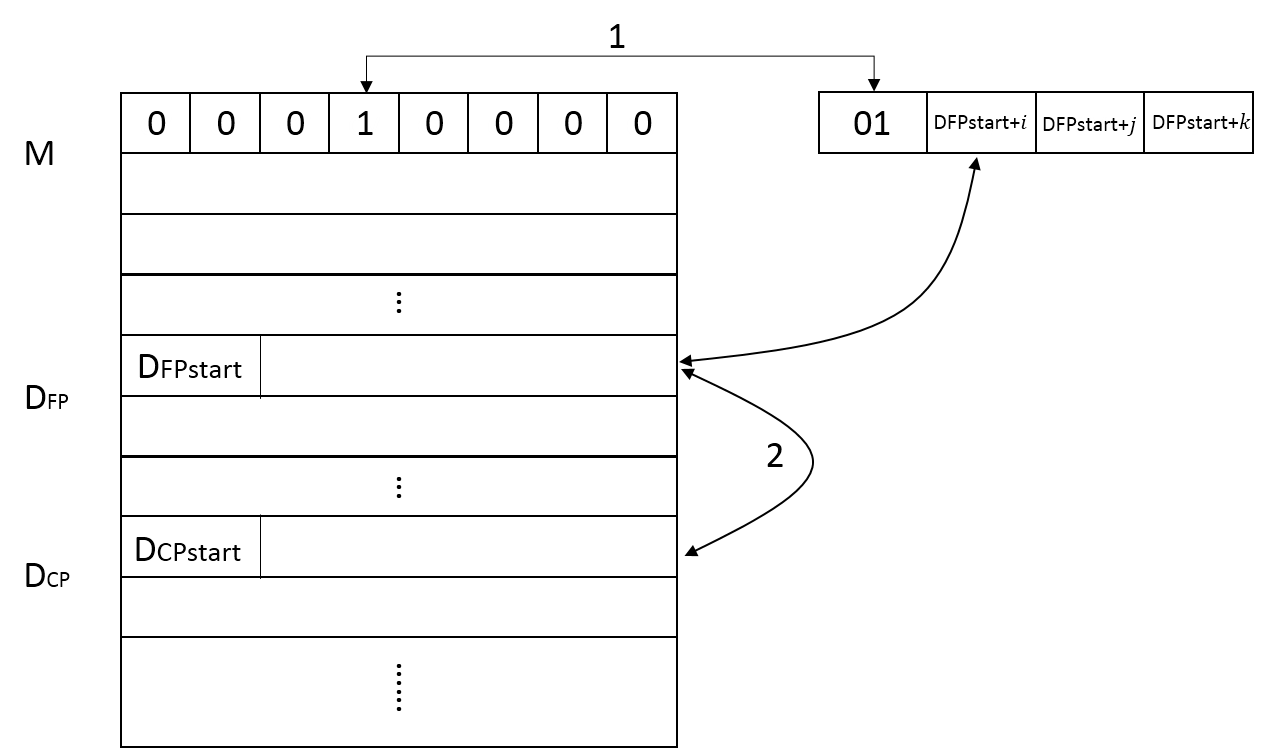
\includegraphics[width=2.5in]{fig/DataTransfer.png}
%	\caption{ The compilation from flexible program to control program}
%	\label{fig:DataTransfer}
%\end{figure}

\begin{figure}
	\centering
	
\includegraphics[width=3in]{fig/execution.png}
	\caption{ The execution OF flexible program}
	\label{fig:execution}
\end{figure}

\subsection{算法层执行}
算法层包含算法层协议解析模块,不断执行解析从控制层传递数据,选择更新算法模块或者执行新的模块。
\subsection{线程运行机制}
通过驱动模块,线程间交互和数据交互实现整个系统的运行。


\section{Case Analysis}
\label{Case}
\subsection{Case 1 双目抛球机器人}
\begin{figure}
	\centering
	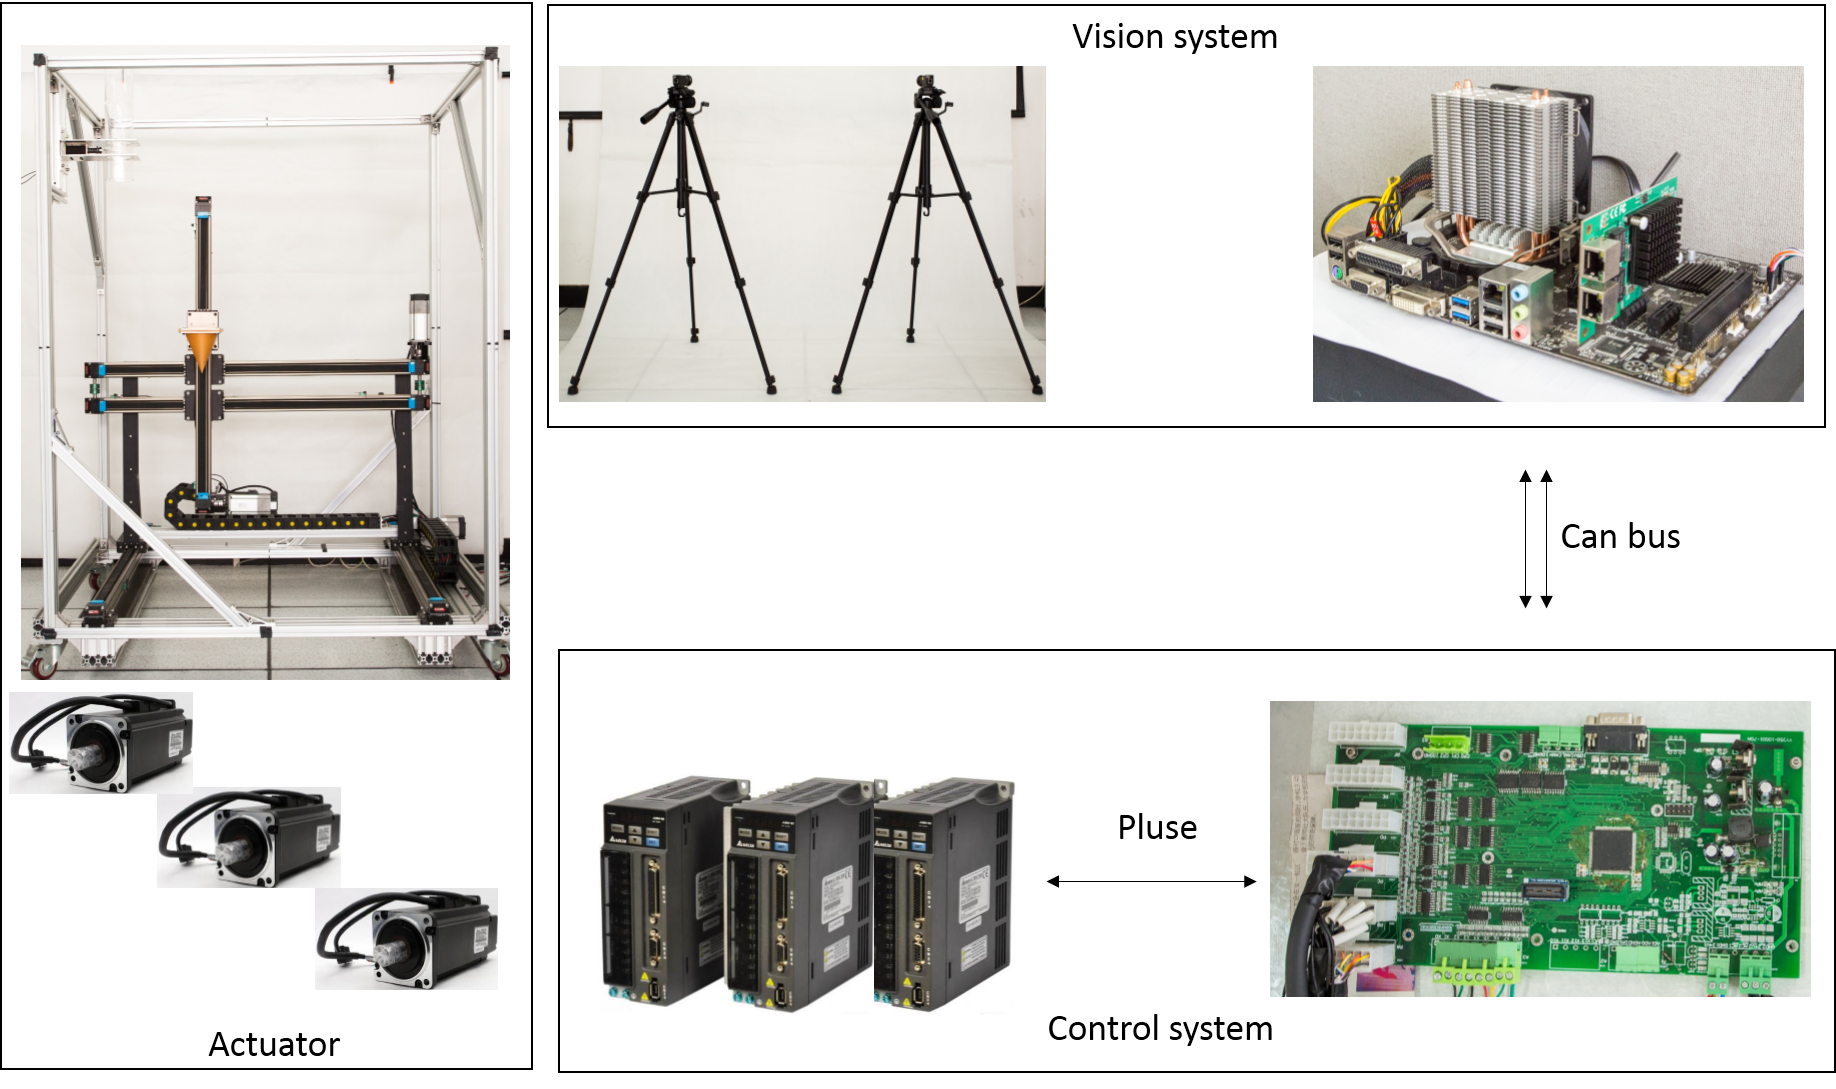
\includegraphics[width=3in]{fig/visual_control_system.png}
	\caption{ Visual servo control system}
	\label{fig:VIsualServoControlSystem}
\end{figure}
\subsubsection{协议设计}

\subsubsection{程序设计}

\subsubsection{运行效果}



\begin{figure}
	\centering
	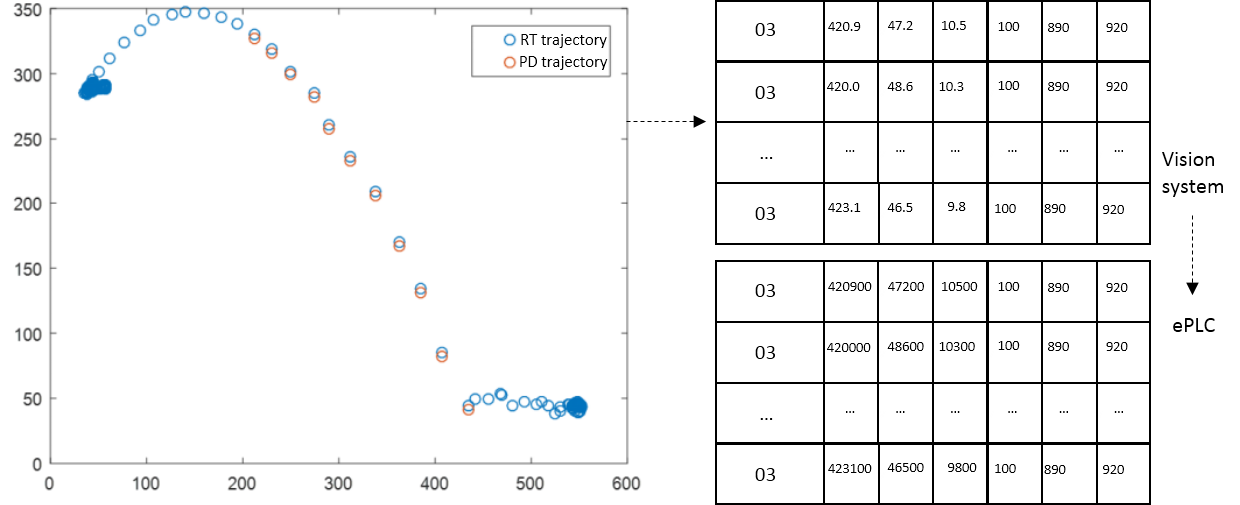
\includegraphics[width=3in]{fig/trajectory.png}
	\caption{ The execution OF flexible program}
	\label{fig:settingexecutionbitinACPTD}
\end{figure}

\subsection{Case 2 带视觉的绕线机}

\subsubsection{协议设计}

\subsubsection{程序设计}

\subsubsection{运行效果}
\begin{figure}
	\centering
	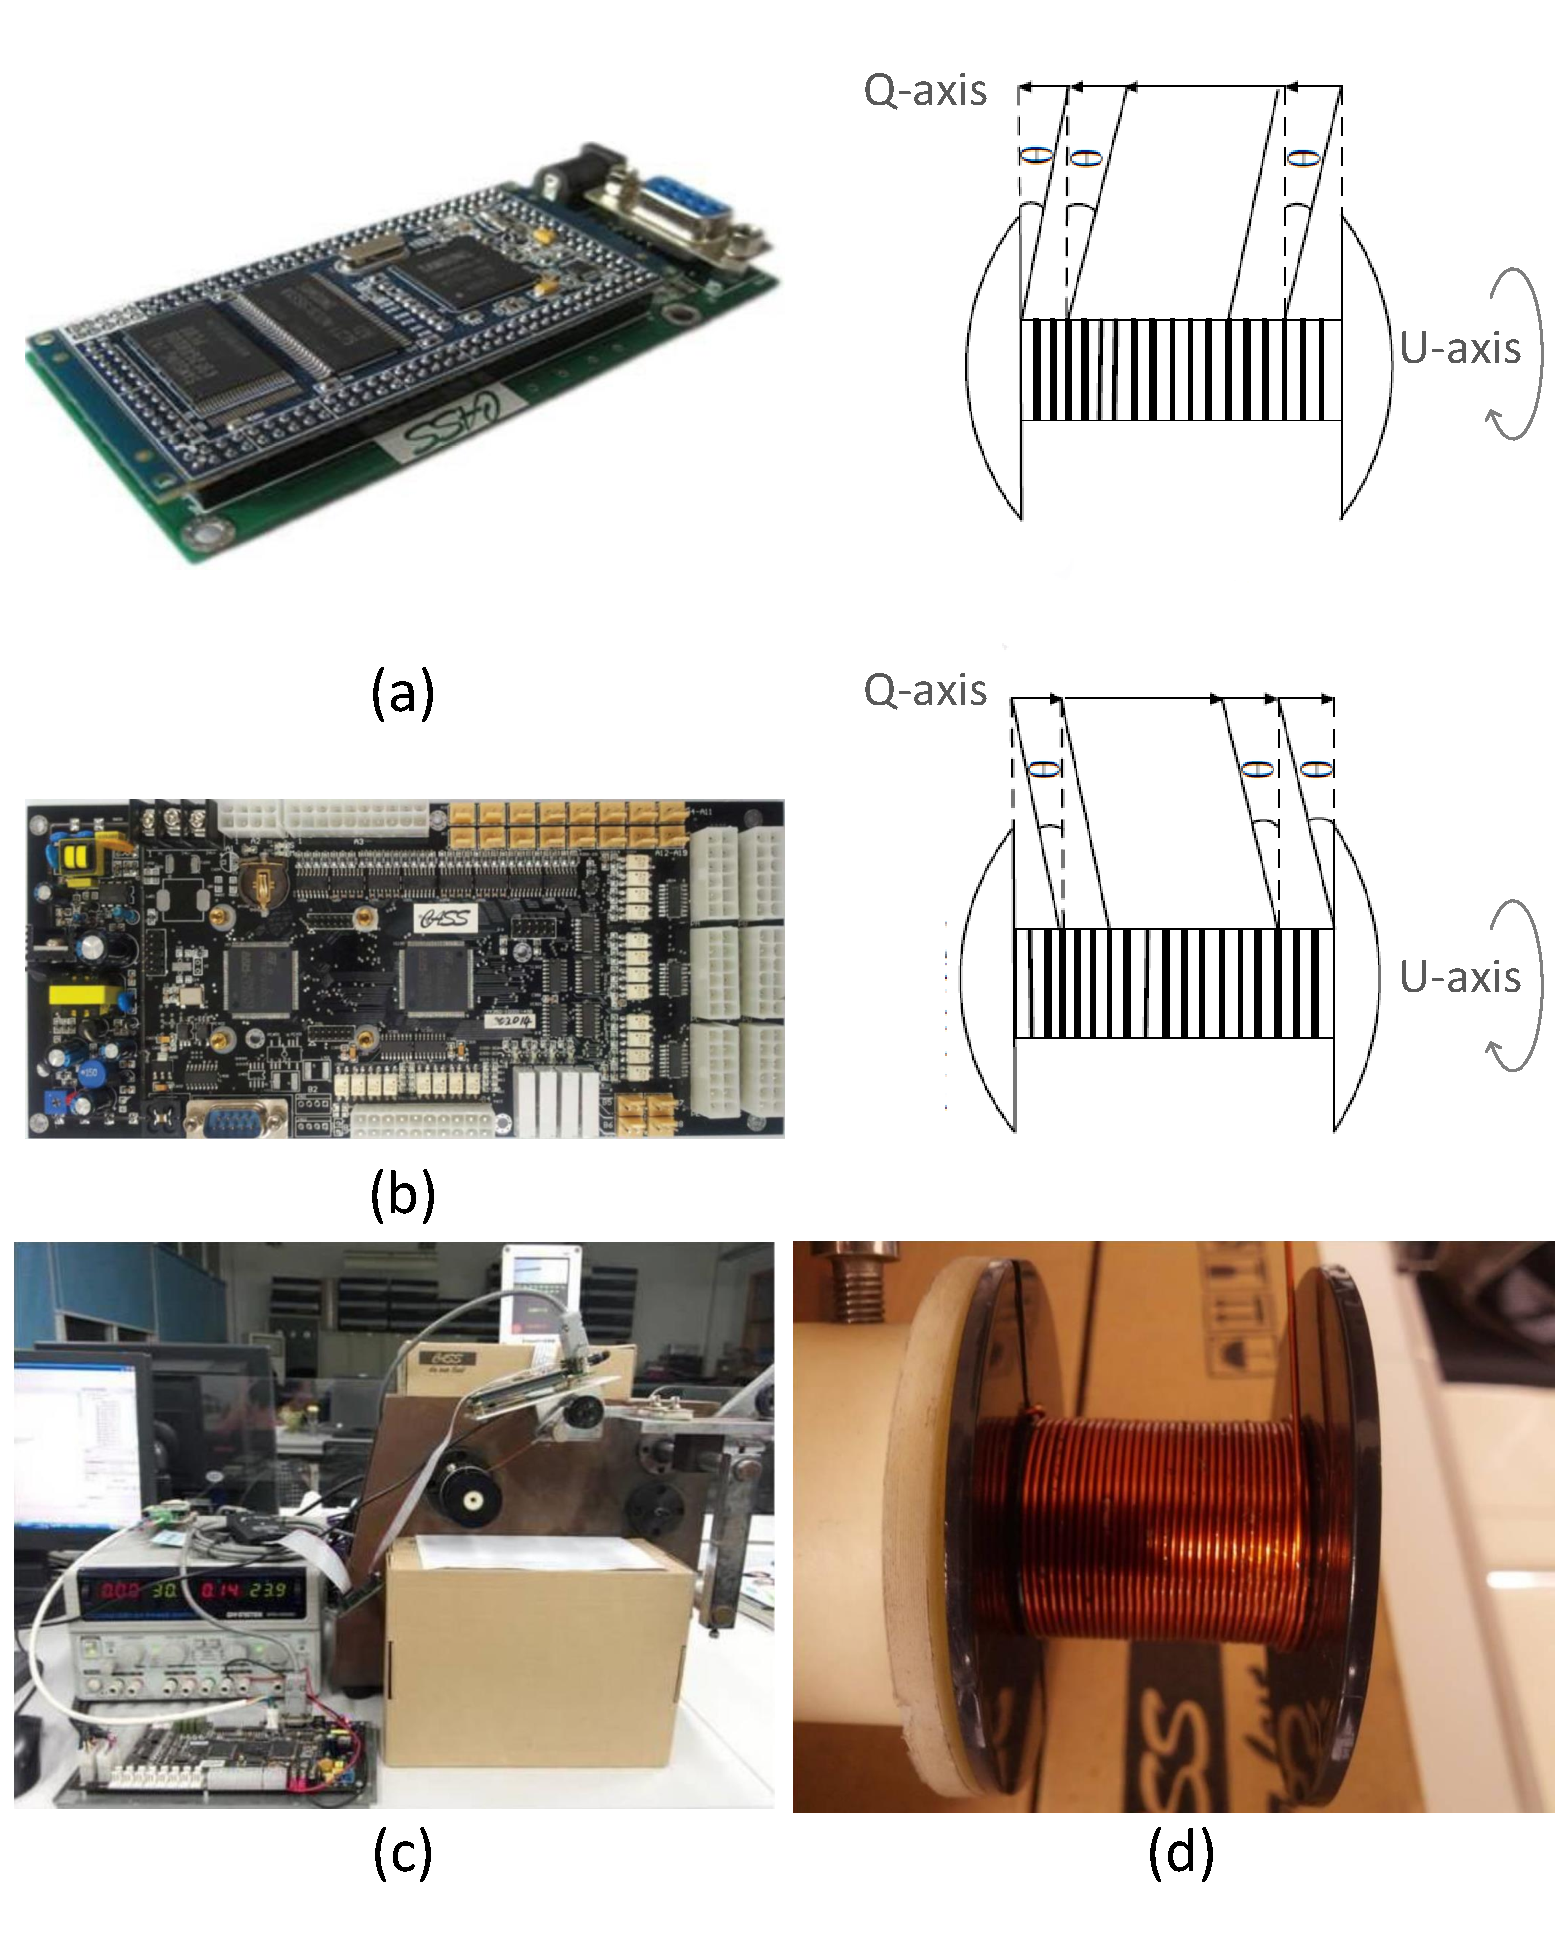
\includegraphics[width=3in]{fig/Winding.pdf}
	\caption{ Winding machine Based on Visual System}
	\label{fig:Winding}
\end{figure}
\section{Conclusion}
\label{conclusion}

下一步我们将实现在PLC开发平台中对逻辑,视觉,运动控制的统一编程,实现支持视觉运动控制的嵌入式PLC。

\ifCLASSOPTIONcaptionsoff
  \newpage
\fi



% trigger a \newpage just before the given reference
% number - used to balance the columns on the last page
% adjust value as needed - may need to be readjusted if
% the document is modified later
%\IEEEtriggeratref{8}
% The "triggered" command can be changed if desired:
%\IEEEtriggercmd{\enlargethispage{-5in}}

% references section

% can use a bibliography generated by BibTeX as a .bbl file
% BibTeX documentation can be easily obtained at:
% http://www.ctan.org/tex-archive/biblio/bibtex/contrib/doc/
% The IEEEtran BibTeX style support page is at:
% http://www.michaelshell.org/tex/ieeetran/bibtex/
%\bibliographystyle{IEEEtran}
% argument is your BibTeX string definitions and bibliography database(s)
%\bibliography{IEEEabrv,../bib/paper}
%
% <OR> manually copy in the resultant .bbl file
% set second argument of \begin to the number of references
% (used to reserve space for the reference number labels box)

\bibliographystyle{IEEEtran}
\bibliography{reference}

% biography section
%
% If you have an EPS/PDF photo (graphicx package needed) extra braces are
% needed around the contents of the optional argument to biography to prevent
% the LaTeX parser from getting confused when it sees the complicated
% \includegraphics command within an optional argument. (You could create
% your own custom macro containing the \includegraphics command to make things
% simpler here.)
%\begin{IEEEbiography}[{\includegraphics[width=1in,height=1.25in,clip,keepaspectratio]{mshell}}]{Michael Shell}
% or if you just want to reserve a space for a photo:

%\begin{IEEEbiography}[{\includegraphics[width=1in,height=1.25in,clip,keepaspectratio]{fig/Author_HuifengWu.eps}}]{Huifeng Wu} received the Ph.D. degree in computer science and technology from Zhejiang university, Hangzhou, China, in 2006. He is currently a professor in the institute of intelligent and software Technology, Hangzhou Dianzi University. His research interests include software development methods and tools, software architecture, embedded system, intelligent control \& automation.
%	
%\end{IEEEbiography}
%\begin{IEEEbiography}[{\includegraphics[width=1in,height=1.25in,clip,keepaspectratio]{fig/Author_YiYan.eps}}]{Yi Yan} received B.S. in automatic control engineering form Zhejiang Sci-Tech University in 1984, M.S. in computer engineering from Beijing University of Postal Telecommunications in 1990. Currently he is the director and full professor in institute of intelligent and software Technology, Hangzhou Dianzi University. His research interests include embedded system, advanced manufacturing system, intelligent control \& automation, and intelligent instruments.
%	
%	
%\end{IEEEbiography}
%\begin{IEEEbiography}[{\includegraphics[width=1in,height=1.25in,clip,keepaspectratio]{fig/Author_DanfengSun.eps}}]{Danfeng Sun} received M.S. in computer architecture from Hangzhou DianZi University in 2011. He is currently a research assistant in the Institute of Industrial Internet, Hangzhou DianZi University. His research interests include embeded system, motion control and IIoT.
%\end{IEEEbiography}
%\begin{IEEEbiography}[{\includegraphics[width=1in,height=1.25in,keepaspectratio,angle=-90]{fig/Author_ReneSimon.eps}}]{Rene Simon} obtained a doctor of engineering at the Otto-von-Guericke University Magdeburg in 2001. He is Professor of Control Systems at the Department of Automation and Computer Sciences, Harz University of Applied Sciences, Wernigerode, Germany. His major research fields include engineering of automation systems, especially industrial controllers. He is chairman of PLCopen and project leader IEC 61131-10 Ed. 1.0.
%\end{IEEEbiography}



% insert where needed to balance the two columns on the last page with
% biographies
%\newpage


% You can push biographies down or up by placing
% a \vfill before or after them. The appropriate
% use of \vfill depends on what kind of text is
% on the last page and whether or not the columns
% are being equalized.

%\vfill

% Can be used to pull up biographies so that the bottom of the last one
% is flush with the other column.
%\enlargethispage{-5in}



% that's all folks
\end{document}


